% !TEX root = ../notes_template.tex
\chapter{Population Dynamics and State-space Models}\label{chp:state_space}

\section{Population Models and Applied Ecology} \label{sec:Chap3_Gompertz}

Population theory (and associated models) are used by applied ecologists working in many different management contexts and for a wide range of taxa.  For example, fisheries managers worldwide set catch quotas based on information from population models \cite{melnychuk_fisheries_2017}.  Similarly, assessments of sustainability inform whether further regulations are needed for many protected species of birds and mammals, and these assessments are based on fitting population models to available data \cite{kery_integrated_2021}.  Furthermore, the dynamics of human or animal disease are often explored by fitting population models to available incidence data \cite{ram_modified_2021}.  

To match this range of taxa and management contexts, population ecologists use a wide range of field, experimental, and analytical methods.  However, these generally involve some combination of:
\begin{enumerate}
    \item \textit{Repeated monitoring}, i.e., field sampling that can record the abundance (number and/or biomass) of an entire population, or some portion that is either representative of the total or of interest by itself.  For example, ecologists count the number of breeding pairs of Adélie penguins in the vicinity of the Palmer Long-Term Ecological Research Station in the Southern Ocean \cite{cimino_long-term_2023};
 
    \item \textit{Information regarding demographic rates and responses}, i.e., using targetted experimental or observation studies to learn about individual demographic processes, such as juvenile survival, growth, maturity, and mortality.  For example, a researcher might conduct a reciprocal transplant experiment to measure how ants adapted to rural or urban environments fair when reared in each of those two habitats, and this might be used to predict changes in demographic rates during continued urbanization \cite{martin_nutshell_2021};
    
    \item \textit{Time-series analysis}, i.e., statistical analysis of abundance from field-sampling, combined with information about demographic rates from targetted studies, which is then fitted as a time-series model.  The resulting analysis could then be used to predict the probability of abundance falling below a minimum threshold (``pseudo-extinction") or, e.g., predict the likely impact of future climate conditions on recovery for southern blue whales given the current moratorium on whaling \cite{tulloch_future_2019}. 
\end{enumerate}
In the following, we use population models to illustrate basic concepts about time-series analysis. We aim to develop familiarity with processes operating over a single dimension (i.e., time), which we can then build upon when introducing two dimensions (e.g., spatial coordinates) or more in later chapters.   

\section{Gompertz Model for Population Dynamics} \label{sec:Chap3_Gompertz_model}

To introduce population-dynamics models, let us assume that we can measure population abundance \(n_t\) in multiple years \(t\) and then calculate the annual population growth rate \( \lambda_t = \frac{n_{t+1}}{n_t} \)\footnote{See https://github.com/james-thorson/Spatio-temporal-models-for-ecologists/Chap\_3 for code associated with this chapter.}.  Ecologists then seek to estimate some function that explains population growth rate, perhaps as a function \(f(.)\) of current population size:

\begin{equation} \label{eq:Chap3_population_dynamics}
    \lambda_t = f(n_{t})    
\end{equation} 
Ecologists often monitor this population growth rate to determine whether trends are sufficient to warrant management changes.  For illustration, we present the simple Gompertz model for population abundance \cite{dennis_estimating_2006}:

\begin{equation} \label{eq:Chap3_Gompertz}
    \lambda_t = e^{\alpha - \beta \log(n_{t})}    
\end{equation} 
This model has several properties that are shared by most population-dynamics models:

\begin{enumerate}
    \item There is some level of population abundance \(K\) (called ``carrying capacity") such that increases and decreases cancel out and the population tends to remain at this level.  Solving \(\lambda_t=1\) for \(n_t\), we see that \( K = e^{\alpha / \beta} \).

    \item The population growth rate can be ``density-dependent", such that an increase in log-abundance decreases population growth by \(\beta\).  
\end{enumerate}

\begin{figure}[!ht]
    \caption[Gompertz model for population dynamics]{Visualizing the growth rate \(\lambda_t\) (y-axis) as a function of abundance \(n_t\) for the Gompertz model of population dynamics, showing that the log-population growth rate is linear with respect to log-abundance (i.e., plotting \(\lambda_t\) and \(n_t\) using log-scale axes as we do here).  Carrying capacity occurs when the growth rate is 1.0 (which occurs here at 3000 animals) and the density dependence is 0.2, suggesting that abundance at half of carrying capacity will have production about 0.2 above replacement.}
    \centering
    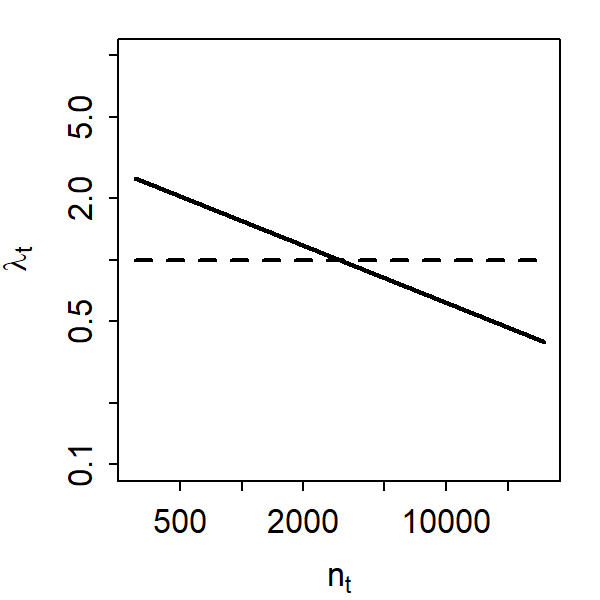
\includegraphics[width=3in]{Chap_3/Gompertz_production.png}
    \label{fig:Chap3_gompertz_production}
\end{figure}

The Gompertz model can be reparameterized such that log-abundance \( \log(n_t) \) in time \(t\) follows a linear model based on log-abundance \( \log(n_{t-1}) \) the year before:

\begin{equation} \label{eq:Chap3_Gompertz_AR1}
    \log(n_{t}) = \alpha + \rho \log(n_{t-1})
\end{equation}
where \( \rho \) is the magnitude of autoregression (Fig. \ref{fig:Chap3_gompertz_production}), and this version is easily converted to the original parameterization in Eq. \ref{eq:Chap3_Gompertz} by setting \( \rho = 1 - \beta \).  Equation \ref{eq:Chap3_Gompertz_AR1} shows that the Gompertz model is a first-order \myindex{autoregressive process} for log-abundance \( \log(n_t) \).  The model has different implications for population dynamics based on the value of \(\rho\):
\begin{itemize}
    \item The population immediately returns to carrying capacity every year when \( \rho=0 \);
    
    \item The population tends to return to its carrying capacity when \( |\rho| < 1 \);
    
    \item The population follows a random walk when \( \rho = 1 \); and
    
    \item The population has oscillatory dynamics when \( \rho<0 \). 
\end{itemize}
This ability to mimic a variety of density-dependent and -independent behaviors has therefore made the Gompertz model a common approach for detecting density dependence across a range of time-series \cite{knape_are_2012}.  

Additionally, we note that the Gompertz model is an approximation to any population model of the form \( x_t = f(x_{t-1}) \) that results in a carrying capacity \(K\).  Specifically, the Gompertz model results from taking the first-order Taylor series expansion of \(f\) with respect to \( \log(n) \) when abundance equals its carrying capacity \(K\).  As expected for a Taylor series expansion, the Gompertz model is ecologically implausible as abundance moves far from where the approximation is calculated (in this case, from carrying capacity).  For example, intrinsic growth rate is often used as a ``common currency" to compare productivity across species, and is typically defined as \(r_0 = \log(\lambda)\) as abundance goes to zero \cite{chesson_mechanisms_2000}.  However, the Gompertz model has an infinite intrinsic growth rate, such that extinction can never occur.  Despite being a poor approximation in these cases, the Gompertz model remains a useful starting point to illustrate time-series analysis of population models.  

Given this simple model, we now proceed to demonstrate several techniques that are useful for population models generally.  In particular, we will:
\begin{enumerate}
    \item fit the model using standard linear estimation methods;

    \item add process errors, and refit the model as a linear state-space model;
    
    \item project the model beyond the range of measurements to illustrate how variance accumulates in time-series dynamics;
    
    \item generalize the Gompertz model to continuous time by briefly introducing a complex and irregular autoregressive process \cite{dennis_density-dependent_2014,elorrieta_discrete-time_2019}.
\end{enumerate}

To start, we fit this model to a multi-decadal time-series of population abundance.  We specifically use data from the Alaska Fisheries Science Center, which has conducted a bottom trawl survey annually following a fixed station design in the eastern Bering Sea using the same survey protocols and gear since 1982 \cite{lauth_results_2016}\footnote{Data are publicly available and were obtained from \url{https://apps-afsc.fisheries.noaa.gov/RACE/groundfish/survey_data/data.htm}.}.  We specifically access data for flathead sole (\textit{Hippoglossoides elassodon}), and this stock supports a substantial commercial fishery with annual landings of approximately 10,000 metric tons \cite{monnahan_assessment_2020}.  To fit this model, we introduce the concept of \myindex{process errors} \( \epsilon_t \).  There is a different estimated value for process errors \(\epsilon_t\) in each year \(t\), and this value represents the net effect of all mechanisms that affect changes in biomass beyond what is predicted by the Gompertz population model. These mechanisms might include age-structured effects, changes in fishery catches, or a nonlinear shape in the function relating biomass changes to current biomass \cite{thorson_bayesian_2014}. We start by assuming that the survey data are a perfect measurement of population biomass, i.e., that there is no measurement error:

\begin{equation} \label{eq:Chap3_process_error_Gompertz}
\begin{gathered}
    \log(b_{t+1}) = \alpha + \rho \log(b_{t}) + \epsilon_{t} \\
    \epsilon_{t} \sim \mathrm{Normal} (0, \sigma_{\epsilon}^2)
\end{gathered}
\end{equation}
where this linear model is then simple to fit in R (Code \ref{code:Chap3-measurement-gompertz}).  The model estimates a carrying capacity of approximately 500,000 tons, i.e., in the right-hand panel of Fig. \ref{fig:Chap3_gompertz_data} as the value of \(b_t\) when the production curve intersects \(\lambda_t=1\).  Similarly, density dependence is significantly different from zero (i.e., the population does not appear to follow a random walk), as shown by the confidence interval for the production curve not including the dotted line showing \(\lambda_t=1\).

\lstset{style=Rcode}
\lstinputlisting[language=R, label=code:Chap3-measurement-gompertz, firstline=32, lastline=41, caption=R code to fit Gompertz dynamics as a linear model., captionpos=t]{Chap_3/Gompertz_dynamics.R}

\begin{figure}[!ht]
    \caption[Abundance for flathead sole using Gompertz process-error model]{The time-series of biomass \(b_t\) (y-axis) over time \(t\) (x-axis) for flathead sole (left panel), and the resulting production \(\lambda_t\) (y-axis) vs. biomass (x-axis) (right panel, where each dot corresponds to \(b_t\) and \(\lambda_t = b_{t+1}/b_t\) in a single year) along with the fitted production curve from a Gompertz model (where the blue shaded area shows the 95\% confidence interval).}
    \centering
    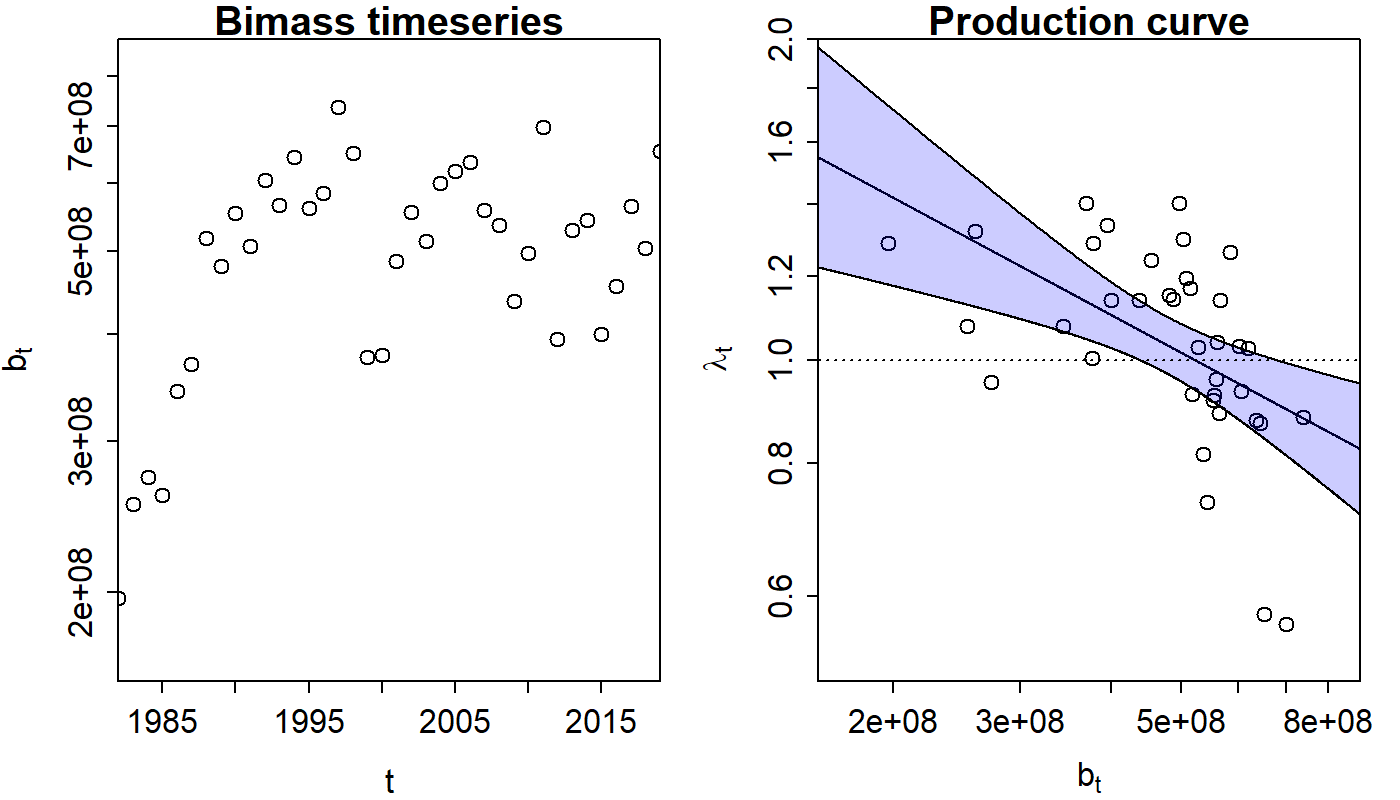
\includegraphics[width=5.5in]{Chap_3/gompertz_data.png}
    \label{fig:Chap3_gompertz_data}
\end{figure}

\section{Semivariance and Correlation Functions} \label{sec:Chap3_semivariance}

Before proceeding further with estimates of population dynamics, we use the Gompertz model to illustrate tools that are useful for understanding or specifying a wide range of spatio-temporal models.  Specifically, we might wonder how much log-abundance \( \log(b) \) is expected to change between two times \(t\) and \(t+\Delta t\).  This can be answered in several ways \cite{cressie_statistics_2011}.

\begin{enumerate}
    \item \textit{Semivariance}:  we can compute the variance of the difference between \( \log(b_t) \) and \( \log(b_{t+\Delta t}) \) for different values \(\Delta t\), and this is called the ``variogram".  However, this difference captures the variance arising at both times, so it is helpful to divide it by two to calculate the \myindex{semivariogram} \(\gamma(\Delta t)\):
\begin{equation}
    \gamma(\Delta t) = \frac{1}{2} \mathrm{Var}( \log(b_t) - \log(b_{t+\Delta_t}) )
\end{equation}
    Many population models are ``stationary" in the sense that the semivariance approaches a plateau (the \myindex{sill} or ``stationary variance") as \( \Delta_t \) increases; 

    \item \textit{Correlation function}: in models with a stationary distribution (i.e., finite sill), we can instead express the similarity between two values as a correlation function \( C(\Delta t) \).  In these cases, it is easy to convert between semi-variance and correlation functions:
\begin{equation}
    C(\Delta_t) = 1 - \frac{\gamma(\Delta t)}{\sigma_{stationary}^2}
\end{equation}
    where \(\sigma_{stationary}^2\) is the stationary variance for a given process.
\end{enumerate}
In later sections, we will often specify a model via the correlation function, because we find it is often more intuitive and simple to explain.  However, the semi-variance remains a more general measurement for autocorrelation, because it applies to both stationary and nonstationary processes (i.e., a random-walk process), while a correlation function can only be defined for stationary processes (i.e., when \(\sigma_{stationary}^2\) can be defined).

\begin{figure}[!ht]
    \caption[Semivariance and correlation for first-order autoregressive process]{The semivariance (top row) and correlation function (bottom row) for a Gompertz population model, calculated either for log-abundance without measurement error (left column, \(\sigma_I^2=0^2\)) or a noisy measurement of log-abundance (right column, \(\sigma_I^2=0.4^2\)), given a constant process errors variance \(\sigma_{\epsilon}^2=0.4^2\) and either moderate (\(\rho=0.5\) in black points) or strong (\(\rho=0.75\) in red points) autocorrelation.}
    \centering
    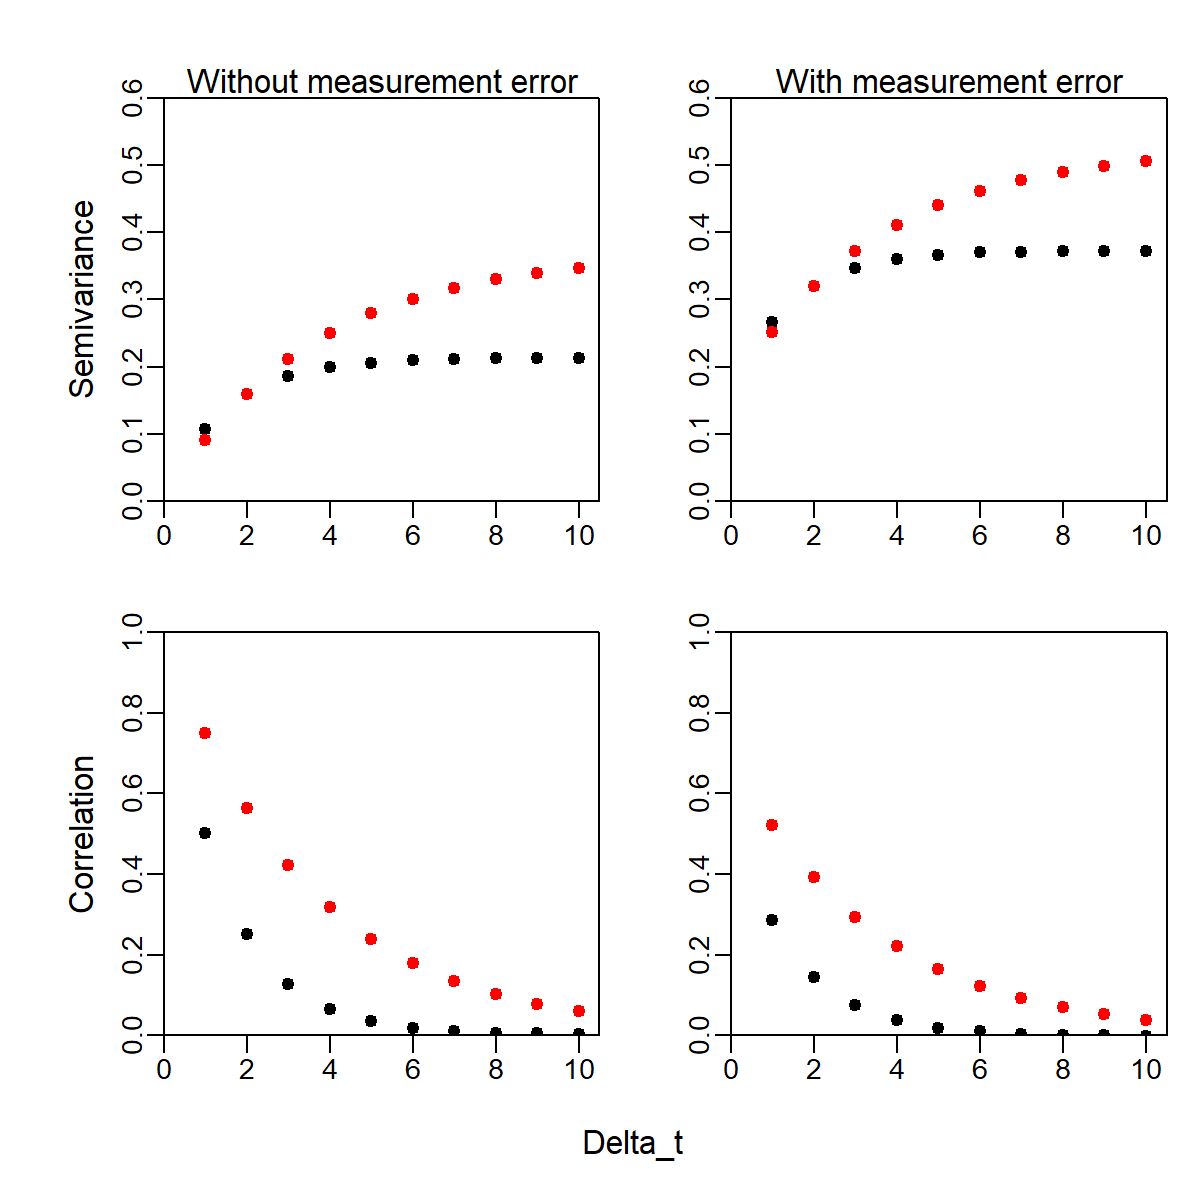
\includegraphics[width=5.5in]{Chap_3/Gompertz_semivariance.png}
    \label{fig:Chap3_semivariance}
\end{figure}

To illustrate these two functions, we simulate the Gompertz model assuming a carrying capacity \(K\) of one million metric tons, calculate the semivariogram and convert it to the correlation function.  We also repeat this with a noisy measurement of abundance \(I_t\), obtained as:

\begin{equation}
    \log(I_t) \sim \mathrm{Normal} (\log(b_{t}), \sigma_{I}^2)
\end{equation}
where \( \sigma_{I}^2 \) is the variance of measurement errors. 
 Results from this simulation experiment (Figure \ref{fig:Chap3_semivariance}) then illustrate a few principles:
\begin{itemize}
    \item Different combinations of autocorrelation \(\rho=\{0.5,0.75\}\) and the magnitude of process errors \(\sigma_{\epsilon}=\{0,0.4\}\) result in a semivariogram that plateaus, such that the Gompertz model is stationary for these tested values.  In fact, the Gompertz model accumulates variance as a power series:
    
\begin{equation} \label{eq:Chap3_AR1_stationary}
    \mathrm{Var}(\log(b_t)) = \sum_{\Delta_t=0}^{\infty} \rho^{2\Delta_t} \sigma_{\epsilon}^2
\end{equation}
    and this power-series is converges if \(|\rho|<1\), such that \(\sigma_{stationary}^2=\sigma_{\epsilon}^2/(1-\rho^2)\);

    \item The time-series that includes measurement errors, \(\log(I_t)\) has higher semivariance for all lags \( \Delta_t \) than a model without measurement errors.  Given the shape of the semivariogram, we could extrapolate its intersection with the y-axis when \(\Delta_t=0\).  This value is sometimes called the \myindex{nugget}, and its value is an estimator for the variance of \myindex{measurement errors} (i.e., the magnitude of variance that would occur if we had replicated but independent samples in a single time);
 
    \item The time-series with higher autocorrelation \(\rho=0.75\), corresponding to weaker density dependence (red points), takes longer to plateau than the time-series with lower autocorrelation \(\rho=0.5\) (black points);

    \item The correlation function for the time-series that does not include measurement errors, \(\log(b_t)\), appears to follow an exponential function, \(C(\Delta_t)=e^{-\rho \Delta_t}\).  The correlation function is in fact easy to calculate for the Gompertz model, but it is sometimes helpful to simulate values from a population model and then calculate the variogram and resulting correlation function for models where an analytical solution is not known.  
\end{itemize}

\section{State-Space Population Model}\label{sec:Chap3_state_space}

Returning to the example for flathead sole in the eastern Bering Sea, we know that the bottom trawl survey has some degree of error in its measurement of total population abundance, both due to limited sample sizes and interannual variation in the vertical and horizontal distribution of fish and resulting availability to the summer survey \cite{oleary_understanding_2022}.  We therefore next fit this model including two sources of variation:
\begin{enumerate}
    \item \textit{Process errors}:  as before, process errors \(\epsilon\) represent a change in biomass beyond what is explained by the Gompertz model, with process-error variance \(\sigma_{\epsilon}^2\); 
    
    \item \textit{Measurement errors}:  however, we also now acknowledge that the survey does not perfectly measure biomass, but instead has some measurement error with variance \(\sigma_I^2\).
\end{enumerate}
Including two sources of variance in a time-series model is conventionally called a \myindex{state-space model}, and estimating parameters requires integrating across one or the other form of variance (either explicitly or implicitly).  Given that this state-space model involves integrating across random effects, we can interpret it as another form of mixed-effect model (see Section \ref{sec:Chap2_why}).   

We can implement this state-space Gompertz population model by specifying:

\begin{equation} \label{eq:Chap3_state_space_Gopmertz}
\begin{aligned}
    \log(b_{t}) & \sim 
    \begin{cases}
        \mathrm{Normal} ( \log(b_0), \sigma_{\epsilon}^2) & \text{if } t=1 \\ 
        \mathrm{Normal} ( \alpha + \rho \log(b_{t-1}), \sigma_{\epsilon}^2) & \text{if } t>1 
    \end{cases} \\
    \log(I_t) & \sim\ \mathrm{Normal} (\log(b_{t}), \sigma_{I}^2)
\end{aligned}
\end{equation}
This model reverts to the previous process-error model (Eq. \ref{eq:Chap3_process_error_Gompertz}) when the variance of measurement errors \(\sigma_I^2 = 0\) is estimated at zero, and reverts to a measurement-error model when the variance of process errors \(\sigma_{\epsilon}^2 = 0\) is estimated at zero.  We could instead parameterize this model by defining process errors \(\epsilon_t\) as a random effect.  As noted in Section \ref{sec:Chap2_Hessian_sparsity}, however, this alternative parameterization results in a less sparse model (i.e., more non-zero elements of the inner Hessian matrix) so we choose instead to treat biomass \(\log(b_t)\) as a random effect.  

Identifying maximum likelihood estimates for parameters \(\theta = \{\alpha,\rho,\log(b_0),\sigma_{\epsilon}^2,\sigma_I^2\}\) while treating \(b_t\) as a random effect in each year involves calculating:

\begin{equation} \label{eq:Chap3_joint_probability}
    \mathcal{L}( \theta; y, x ) = \int e^{f(x,\theta,y)} \mathrm{d}x 
\end{equation}
where \( f(x,\theta,y) = \log (\Pr(y | \theta, x)) + \log (\Pr( x | \theta)) \) and we change variables \( x_t = \log(b_t) \) and \( y_t = \log(I_t) \) to allow compact notation. We then factor the joint probability of random effects \( \Pr( x | \theta) \) into a series of separable conditional distributions:

\begin{equation} \label{eq:Chap3_factored_probability}
    \log(\Pr(x|\theta)) = \log (\Pr( x_1 )) + \log (\Pr( x_2 | x_1 )) + ... + \log (\Pr( x_T | x_{T-1} ))
\end{equation}
where we drop the dependency upon \(\theta\) on the right-hand-side for simplicity of notation. The joint distribution (Eq. \ref{eq:Chap3_joint_probability}) can be factored into these conditional probabilities (Eq. \ref{eq:Chap3_factored_probability}) because the Gompertz model has a 1st-order \myindex{Markov structure}, wherein the probability for state \(x_t\) depends only on its value in the immediately preceding time \(x_{t-1}\).   

\begin{figure}[!ht]
    \caption[Graphical model for first-order autoregressive process]{A graphical model for the first four years in our Gompertz conditional autoregressive model, showing data \(y_t = \log(I_t)\) as boxes, random effects \(x_t = \log(b_t)\) as diamonds, and fixed effects \(\{\alpha,\rho,\log(b_0)\}\) as circles (while dropping variance parameters \(\{\sigma_{\epsilon}^2,\sigma_I^2\}\) for visual clarity), and showing the conditional dependencies as arrows.}
    \centering
    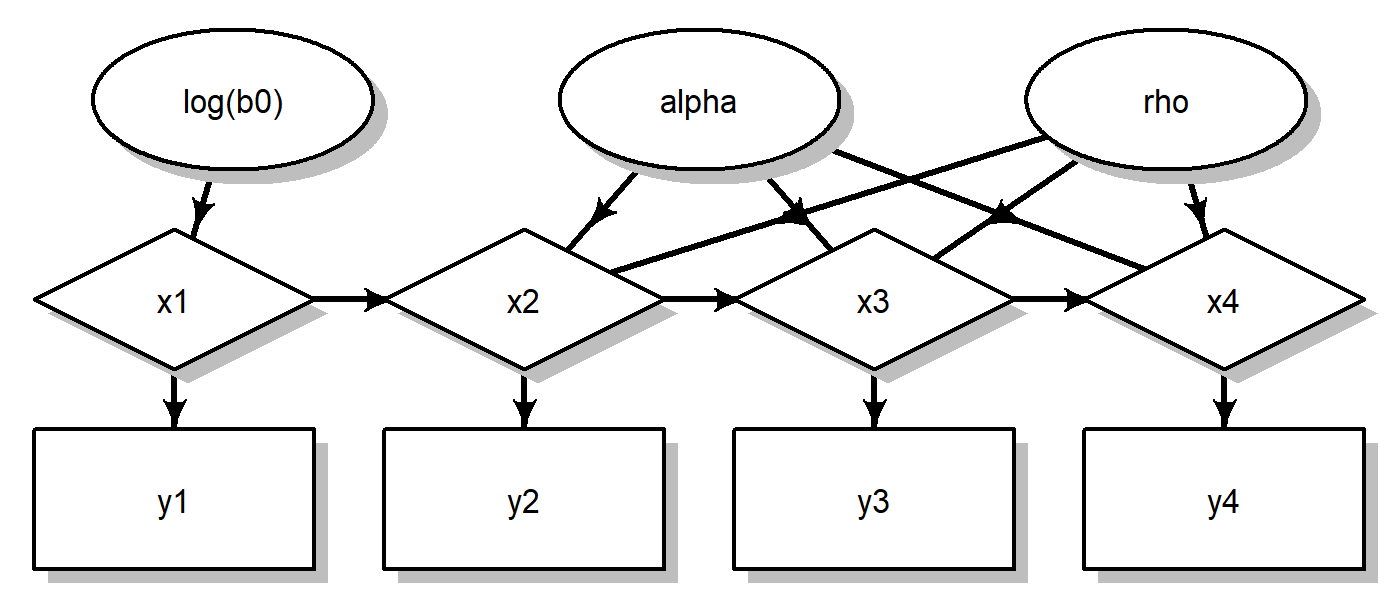
\includegraphics[width=5.5in]{Chap_3/graph.png}
    \label{fig:Chap3_gompertz_graph}
\end{figure}
From this factored version, we can see that \(x_{t+1}\) is statistically independent of \(x_{t-1}\) conditional upon the value of \(x_t\).  In the graphical representation (Fig. \ref{fig:Chap3_gompertz_graph}), this is seen where random effects \(x_1\) and \(x_3\) do not both connect to any single datum (box), and are also not connected directly by any arrow, and hence expect that the inner Hessian should be sparse (recall rules from Section \ref{sec:Chap2_Hessian_sparsity}).  Alternatively, we can express this as a \myindex{simultaneous autoregressive process} (SAR), and see Appendix \ref{sec:Appendix_SAR} for more details.  

\lstset{style=TMBcode}
\lstinputlisting[language=c++, label=code:Chap3-TMB-state-space, caption=TMB code to specify a state-space Gompertz model., captionpos=t]{Chap_3/gompertz.cpp}

Coding this joint negative log-likelihood in TMB involves specifying fixed and random effects, and we follow Eq. \ref{eq:Chap3_state_space_Gopmertz} in defining log-biomass \colorbox{backblue}{log\_d\_t} as a coefficient that we will then specify as a random effect (Code \ref{code:Chap3-TMB-state-space}).  We also include additional code (i.e., lines using the \colorbox{backblue}{SIMULATE} function) that we will discuss in detail in a later section. Fitting this model in R is similarly straightforward (Code \ref{code:Chap3-R-state-space}), given that TMB will calculate the marginal likelihood (i.e., apply the inner optimizer and calculate the Laplace approximation) automatically. 

\lstset{style=Rcode}
\lstinputlisting[language=R, label=code:Chap3-R-state-space, firstline=136, lastline=149, caption=R code to run the state-space Gompertz model implemented in TMB., captionpos=t]{Chap_3/Gompertz_dynamics.R}

\begin{figure}[!ht]
    \caption[Sparsity pattern for first-order autoregressive process]{Sparsity pattern of the inner Hessian for the state-space Gompertz model, showing that random effects are conditionally independent for any two years that are not adjacent.}
    \centering
    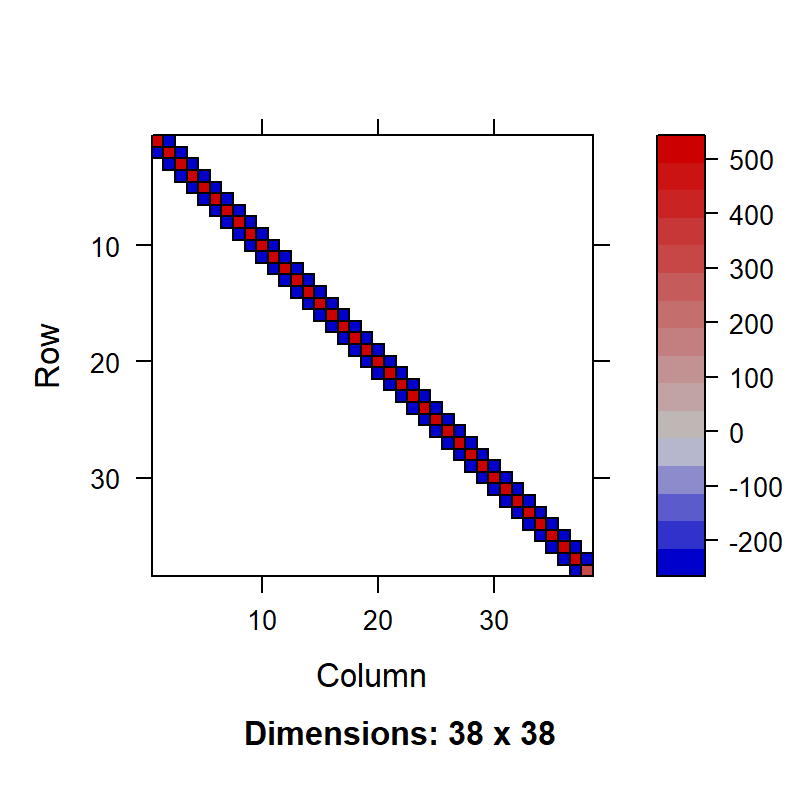
\includegraphics[width=3in]{Chap_3/gompertz_sparsity.png}
    \label{fig:Chap3_hessian}
\end{figure}

Before running the model, however, we check the sparsity of the inner Hessian to confirm that we have used an efficient parameterization (Fig. \ref{fig:Chap3_hessian}). As expected for a first-order Markov process, this shows that we have used a parameterization whereby the distribution for \(\log(b_{t+1})\) is independent of \(\log(b_{t-1})\) conditional upon the value of \(\log(b_{t})\).  Finally, we run the model and estimate uncertainty in both biomass and the production function:

\begin{figure}[!ht]
    \caption[Biomass estimated using conditional autoregressive model]{The time-series of the biomass index for flathead sole in the eastern Bering Sea (left panel) along with estimated biomass (red line, with red shading showing the 95\% confidence interval), and the resulting production (where each dot corresponds to \(b_t\) and \(\lambda_t = b_{t+1}/b_t\) in a single year) along with the fitted production curve from a Gompertz model (blue line, with blue shading showing the 95\% confidence interval), which can be compared with Fig. \ref{fig:Chap3_gompertz_data}.}
    \centering
    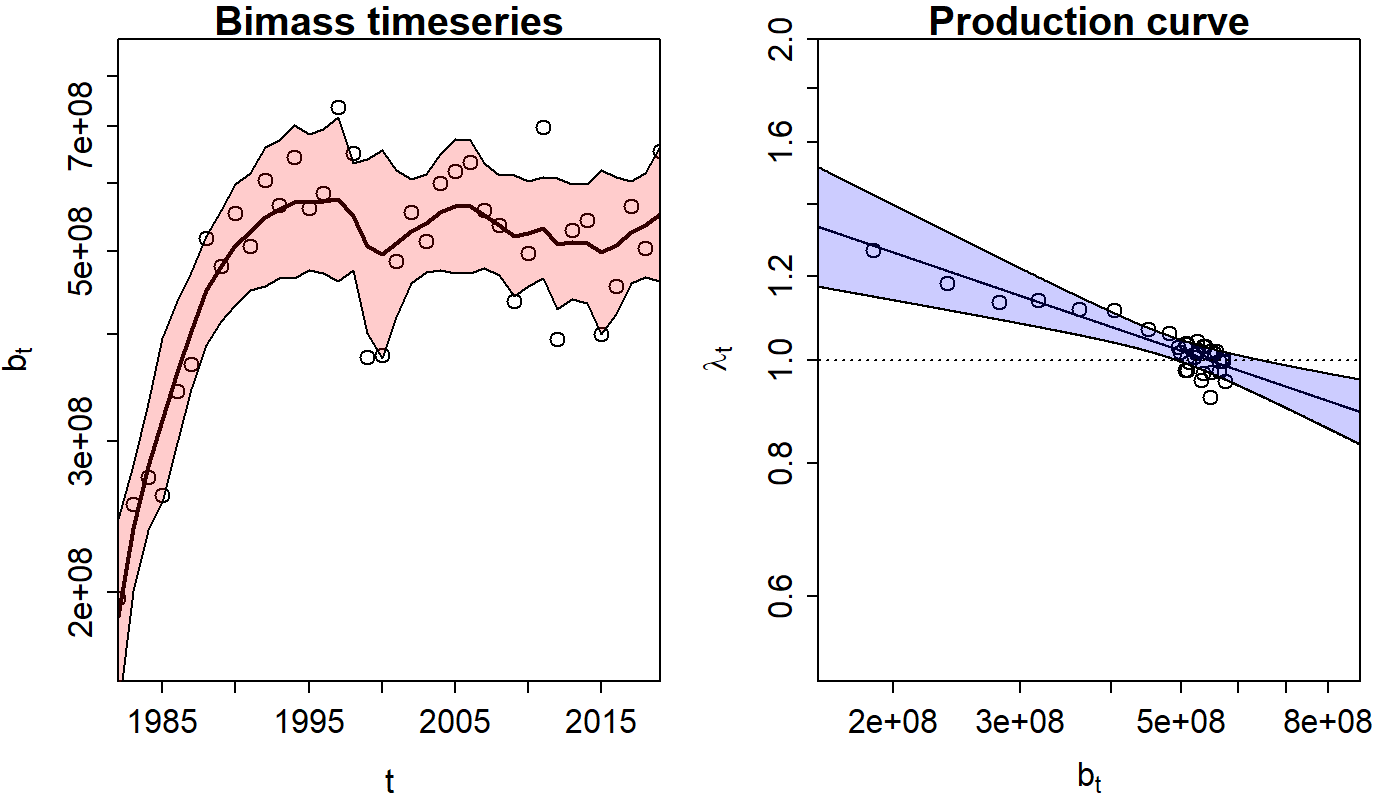
\includegraphics[width=5.5in]{Chap_3/gompertz_fit.png}
    \label{fig:Chap3_gompertz_conditional}
\end{figure}

Comparing the state-space (Fig. \ref{fig:Chap3_gompertz_conditional}) and process-error 
models (Fig. \ref{fig:Chap3_gompertz_data}) shows that the state-space model estimates a true but unobserved time-series of biomass that is more smooth than the survey observations, and also estimates population growth rates that are shrunk toward the predictions from the Gompertz population model.  As introduced in Section \ref{sec:Chap2_why}, we expect that this shrinkage estimator for biomass will have lower expected error than using the raw survey data as an estimate of population biomass.  Similarly, the estimated magnitude of process and measurement errors determines how much biomass is shrunk (left-hand side of Fig. \ref{fig:Chap3_gompertz_conditional}) relative to how much production is shrunk toward the Gompertz model (right-hand side of Fig. \ref{fig:Chap3_gompertz_conditional}).  

\section{Conditional vs. Joint Covariance Modeling} \label{sec:Chap3_joint_Gompertz}

So far in this chapter, we have developed the state-space Gompertz model for population dynamics by factoring the joint log-likelihood into a series of conditional log-likelihood components (Eq \ref{eq:Chap3_factored_probability}). We then code that expression in TMB, and TMB assembles a graph representing the dependency among variables and data, which is conceptually similar to the graphical model in Fig. \ref{fig:Chap2_graph}.  TMB uses this graph and applies a feature called \myindex{automatic sparseness detection} to identify all pairs of random effects that are conditionally independent of one-another, and hence detect the sparsity of the resulting Hessian matrix (e.g., in Fig. \ref{fig:Chap3_hessian}).  As we will see, automatic sparseness detection is extremely handy for most users, who then do not have to manually specify which random effects are conditionally independent.

In some cases, however, it is helpful to understand alternative approaches to implementing this same model, which provide different statistical insights or options for writing code.  Here, we next reparameterize this model by simultaneously calculating the probability of all random effects, i.e., calculating \( \Pr(\mathbf{b}) \) directly.  We seek to show that both versions give nearly identical parameter estimates.  In later chapters, we will often introduce a model by expressing the probability of random effects using a series of conditional distributions, because we find that this derivation is often more intuitive.  We will then sometimes replace this specification with a joint distribution, which can often be written using fewer lines of code and hence is easier to read and maintain as software.  We therefore think that both versions can be useful in different circumstances.  

The joint version of the Gompertz model \cite{thorson_importance_2014} is written as:
\begin{equation}
\begin{aligned}
    \log(\mathbf{b}) & = \log(b_0) \rho^{\mathbf{t}} + \frac{\alpha}{1-\rho} + \mathbf{\epsilon} \\
    \mathbf{\epsilon} & \sim \mathrm{MVN} (\mathbf{0}, \sigma_{\epsilon}^2 \mathbf{R}_{\epsilon}) \\
    \log(I_t) & \sim \mathrm{Normal} (\log(b_{t}), \sigma_{I}^2) 
\end{aligned}
\end{equation}
where \(\log(b_0)\) is the initial log-biomass in time \(t_0\) relative to car, which follows an exponential decay toward carrying capacity as time increases, \(\mathbf{t} = \{0,1,...,T-1\}\) is the vector of times after the initial modeled interval, such that \(\rho^{\mathbf{t}}\) is the amount that initial biomass has decayed by each time \(\mathbf{t}\).  Additionally, \( \mathbf{\epsilon} \sim \mathrm{MVN} \) indicates that \( \mathbf{\epsilon}\) follows a multivariate normal distribution, \(\mathbf{0}\) is a vector of \(T\) zeros, and \( \mathbf{R}_{\epsilon} \) is a \(T\) by \(T\) matrix containing the correlation in \(\epsilon_t\) between any two times \(t_1\) and \(t_2\):

\begin{equation}
    r_{t_1,t_2} = \rho^{|t_2-t_1|}
\end{equation}
such that:

\begin{equation} \label{eq:Chap3_joint_correlation}
    \mathbf{R}_{\epsilon} = \begin{bmatrix}
    1 & \rho^1 & \rho^2 & \rho^3 \\
    \rho^1 & 1 & \rho^1 & \rho^2 \\
    \rho^2 & \rho^1 & 1 & \rho^1 \\
    \rho^3 & \rho^2 & \rho^1 & 1\\
    \end{bmatrix} 
\end{equation}
This correlation matrix is dense, i.e., has a nonzero value everywhere.  However, recall from Section \ref{sec:Chap2_Laplace} that calculating the multivariate normal distribution (Eq. \ref{eq:Chap2_MVN}) only requires knowing the inverse of the covariance \( \mathbf{Q}_{\epsilon} = (\sigma_{\epsilon}^2 \mathbf{R})^{-1} \), called the ``precision matrix" \cite{rue_gaussian_2005}.  Conveniently, this precision matrix is sparse and can be approximated (while ignoring small differences at the beginning of the time-series which we call \myindex{boundary conditions}) as:

\begin{equation} \label{eq:Chap3_joint_precision}
    \mathbf{Q}_{\epsilon} = (\sigma_{\epsilon}^2 \mathbf{R}_{\epsilon})^{-1} = \sigma_{\epsilon}^{-2} \begin{bmatrix}
    1+\rho^2 & -\rho & 0 & 0 \\
    -\rho & 1+\rho^2 & -\rho & 0 \\
    0 & -\rho & 1+\rho^2 & -\rho \\
    0 & 0 & -\rho & 1+\rho^2 \\
    \end{bmatrix}
\end{equation}
In fact, this sparse form matches the ``tri-diagonal" form of the inner Hessian matrix that was seen earlier for the factored version of the Gompertz model (Figure \ref{fig:Chap3_hessian}).  Interested readers can see Appendix \ref{sec:Appendix_SAR} for more information on deriving \ref{eq:Chap3_joint_precision} for the Gompertz model.

\lstset{style=TMBcode}
\lstinputlisting[language=c++, label=code:Chap3-TMB-density-namespace, caption=TMB code to fit a state-space Gompertz model by constructing an AR1 precision matrix and then using the \colorbox{backblue}{density} namespace to evaluate the multivariate normal density function., captionpos=t]{Chap_3/gompertz_SAR.cpp}

We can therefore implement this joint version of a Gompertz population model in TMB by calculating the precision matrix as a sparse matrix using the C++ package \colorbox{backblue}{Eigen}.  The \colorbox{backblue}{Eigen} package requires some special syntax, e.g., using \colorbox{backblue}{Q$.$coefRef(a,b)$=$c} to assemble the triplet-format precision matrix where row \colorbox{backblue}{a} and column \colorbox{backblue}{b} of matrix \colorbox{backblue}{Q} has value \colorbox{backblue}{c}.  We then use a built-in package \colorbox{backblue}{density} in TMB to calculate the multivariate normal distribution using this precision matrix (Code \ref{code:Chap3-TMB-density-namespace}). Comparing the maximum likelihood estimates of parameters for the conditional and joint versions shows some small differences, resulting from a different treatment of boundary conditions for random effects (Table \ref{tab:Chap3_conditional_and_joint}).  However, these differences have little effect on resulting estimates of biomass or the production function (Figure \ref{fig:Chap3_gompertz_simultaneous}).

\begin{table}
  \caption[Comparing estimates between conditional and joint covariance models]{Estimated parameters and standard errors for the Gompertz population model using a conditional or joint specification of the covariance.}
  \catcode`"=9
  \centering
    \csvreader[
      tabular=|c|r|r|c|r|r|,
      table head=\hline \bfseries{CAR param} & \bfseries{Estimate} & \bfseries{Std. Error} & \bfseries{SAR param} & \bfseries{Estimate} & \bfseries{Std. Error} \\\hline,
      late after last line=\\\hline % horizontal line at the end of the table
    ]{Chap_3/TMB_comparison.csv}{}{\csvlinetotablerow}
  \label{tab:Chap3_conditional_and_joint}
\end{table}

\begin{figure}[!ht]
    \caption[Biomass estimated using simultaneous covariance for model]{Output from the joint implementation of the Gompertz population model (see Figure \ref{fig:Chap3_gompertz_conditional} for details).}
    \centering
    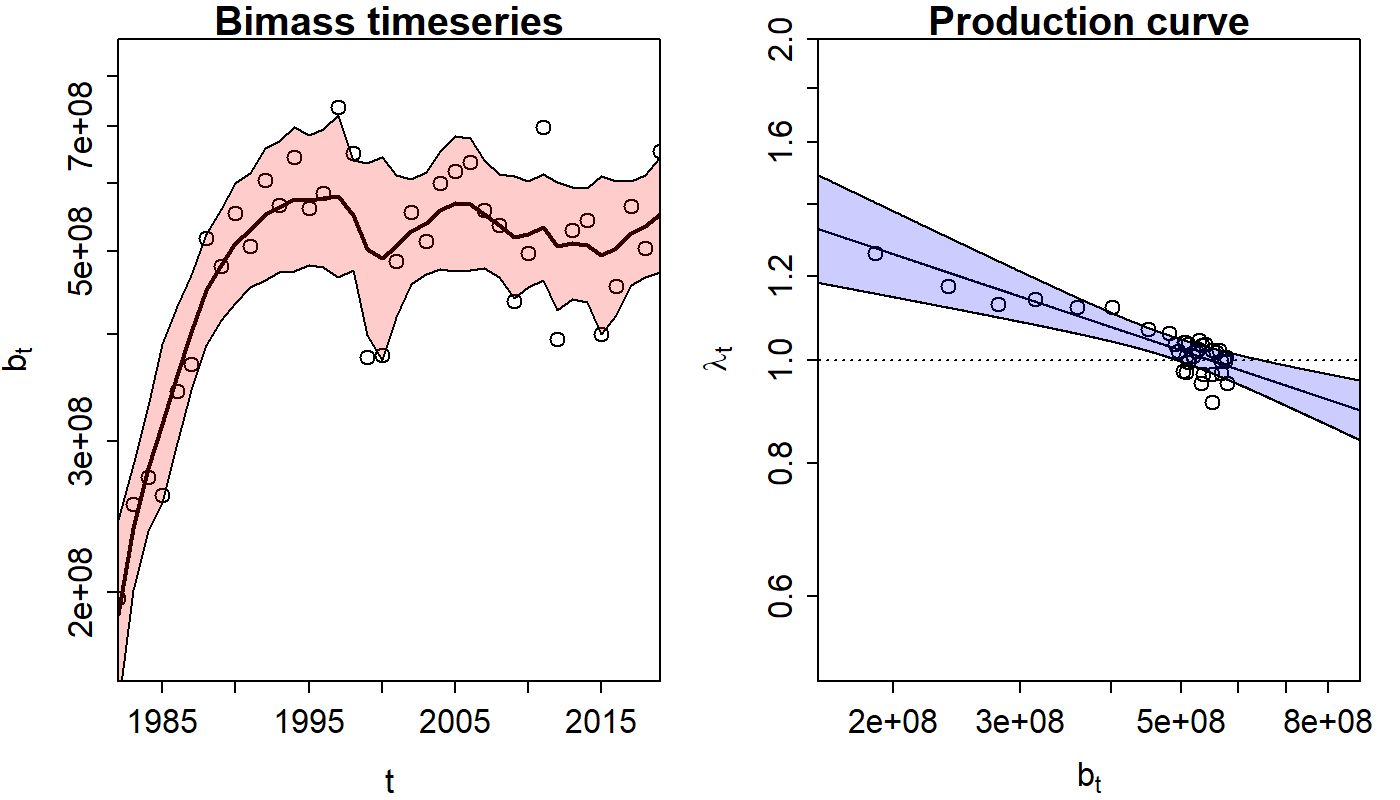
\includegraphics[width=5.5in]{Chap_3/gompertz_fit_SAR.png}
    \label{fig:Chap3_gompertz_simultaneous}
\end{figure}

\section{Seasonal/missing Data and Forecasting} \label{sec:Chap3_seasonal}

So far, we have shown how to implement a state-space population-dynamics model using either conditional or joint specification of the covariance among states \( \log(b_t)\).  We next summarize how this is generalized to deal with several practical issues that arise in ecological time series, namely:
\begin{enumerate}
    \item \textit{Seasonal data}: how can we deal with data that arise irregularly, i.e., by defining a process in continuous time?

    \item \textit{Missing data}: how can be fit models when data are missing for some times?

    \item \textit{Forecasting}: how can we forecast dynamics into the future?
\end{enumerate}

First, we might have irregularly spaced samples of population dynamics.  For example, the bottom trawl survey in the eastern Bering Sea typically occurs with midpoint in July but ranges from June to August depending upon logistical constraints in each year.  Therefore, instead of indexing time as an integer \( t \in \{1,2,...,n_t\} \), we might define time as a continuous variable \( t_{min} \leq t \leq t_{max} \).  In this case, we replace the autoregressive model (Eq. \ref{eq:Chap3_process_error_Gompertz}) with a generalization called an \index{irregular autoregressive model}\textit{irregular autoregressive (IAR) model}.  This IAR model specifies \( \log(b_{t+\Delta_t}) \) based on the continuous-valued time \(\Delta_t\) elapsed since the previous observation:

\begin{equation} \label{eq:Chap3_IAR}
\begin{gathered}
    \log(b_{t+\Delta_t}) = (1-\rho^{\Delta_t}) \frac{\alpha}{1-\rho} + \rho^{\Delta_t} \log(b_t) + \epsilon_t \\
    \epsilon_t \sim \mathrm{Normal}(0, \sigma_{\epsilon}^2 \sqrt{1-\rho^{2 \Delta_t}})
\end{gathered}
\end{equation}
where the autocorrelation, intercept and standard deviation variance of \(\epsilon\) all depend upon the time elapsed.  Notably, the autocorrelation parameter \(\rho\) is now defined as the correlation for a reference time-interval.  This continuous-time model could then be fitted to samples \(I(t)\) in each of those times.  This IAR can instead be parameterized as an \myindex{Ornstein-Uhlenbeck process} by replacing \( \rho = e^{-\theta} \) \cite{dennis_density-dependent_2014}, although we present the IAR to highlight the similarity to Eq. \ref{eq:Chap3_state_space_Gopmertz}.   

In Section \ref{sec:Chap3_joint_Gompertz}, we discussed how the Gompertz model with equal time-intervals can be parameterized by either specifying (1) the conditional distribution for biomass \(b_t\) at each time given the previous \(b_{t-1}\), or (2) the distribution for biomass \(\mathbf{b}\) for all times jointly.  In Eq. \ref{eq:Chap3_IAR}, we use the former \textit{conditional specification} but we could instead use the latter \textit{joint specification} for the IAR model (which we later recommend as an Exercise for the reader).  We can therefore interpret this IAR as a \myindex{Gaussian process}, which defines a probability distribution for the biomass function \(b(t)\) at any continuous time \(t\), such that biomass for any finite set of times will follow a multivariate normal distribution \cite{rasmussen_gaussian_2006}.  In later chapters, we will repeatedly define a multivariate normal distribution for process errors across space and/or time.  In many cases, a set of spatially or temporally varying random effects that follows a joint multivariate normal distribution can be viewed as a draw from a Gaussian process, and the model can be viewed as a distribution for a function-valued variable \cite{thorson_using_2017}.

The autocorrelation for the IAR in Eq. \ref{eq:Chap3_IAR} is constrained to be positive, but otherwise the model reduces to the equal-interval Gompertz model (Eq. \ref{eq:Chap3_process_error_Gompertz}) when time intervals \(\Delta_t\) are constant, and parameters are identical with appropriate rescaling of \( \Delta_t=1 \).  As a further extension, we could instead use a \myindex{complex irregular autoregressive model} (CIAR).  This CIAR \cite{elorrieta_discrete-time_2019} represents oscillatory time-series dynamics by introducing a latent variable representing the momentum in the rate of population change, analogous to the momentum of a pendulum that results in its oscillatory movement.  Viewed more formally, we can model the state-variable as a \textit{complex number} \( x = y + zi \), where real component \(y\) and imaginary component \(z\) both follow an IAR, but we only observe the real component of this variable which is then interpreted as log-biomass \(y = \log(b)\).  Treating the state-variable as a complex number allows an autoregressive model for \(\log(b)\) to include oscillations, where the expected frequency arises from estimated parameters, similar to the original oscillatory dynamics that arise in the equal-interval Gompertz model whenever \(\rho < 0\).

Similarly, it is easy to calculate the Gompertz model with missing data: this simply involves excluding any data that are missing from the calculation of the joint loglikelihood function (which we accomplished using \colorbox{backblue}{R\_IsNA} in Code \ref{code:Chap3-TMB-state-space}).  However, the performance of the state-space model will likely change as data are progressively removed. To illustrate this, let's start by supposing we have a model where the state-space Gompertz model can be fitted using maximum likelihood, where both variance parameters \( \hat{\sigma}_P\) and \(\hat{\sigma}_M\) are estimated to be greater than zero.  As data are removed, one or the other of these parameters will often be estimated at zero, corresponding to a model that includes only measurement or process variability.  In this case, the state-space model is not ``estimable" (see Section \ref{sec:Chap2_outer_hessian_failure}), and the model instead collapses to a simpler model without measurement errors (\(\sigma_I=0\)) or process errors (\(\sigma_{\epsilon}=0\)).  

Finally, ecologists often seek to project likely population dynamics into the future.  However, population projections are uncertain for several important reasons:
\begin{enumerate}
    \item \textit{Parametric uncertainty}\index{parametric uncertainty}: typically, we are uncertain about the parameters representing population dynamics, and forecasts using different values will result in different dynamics.  We can measure this uncertainty by the standard errors of fixed effects;

    \item \textit{Uncertainty about historical states}\index{uncertainty about historical states}: similarly, forecasts are initialized based on the population abundance in the final year of data. This population abundance is typically uncertain, and uncertainty about initial conditions will then propagate forward during forecasts.  We can measure this uncertainty using the predictive variance of random effects representing historical biomass;

    \item \textit{Future variability}\index{future variability}:  finally, the state-space Gompertz model identifies process errors, representing the cumulative impact of unknown factors that affect population dynamics. We can measure this uncertainty using the predictive variance of random effects that occur during the forecast period.
\end{enumerate}
Different combinations of these are more or less easy to extract using previous TMB code (Code \ref{code:Chap3-TMB-state-space}) and compact code in R (Code \ref{code:Chap3-forecast-variance}).  For example:
\begin{itemize}
    \item \textit{Total uncertainty}:  We can calculate the net effect of all forms of variability by including future years but treating them as missing data (i.e., using \colorbox{backblue}{R\_IsNA} to skip data that are inputted as NAs).  We then use \colorbox{backcolour}{TMB::sdreport} to calculate standard errors for biomass in those forecasted years;

    \item \textit{Future variability}:  We can isolate the effect of uncertainty about future process errors by including the \colorbox{backblue}{SIMULATE} function in the TMB file to simulate new values for random effects that occur during the forecast period (where we identify which years to resimulate using the vector \colorbox{backblue}{simulate\_t}), but otherwise leaving the fixed and other random effects at their estimated values;

    \item \textit{Uncertainty about historical states}:  We can approximate the effect of uncertainty about historical states by taking random draws from the precision of random effects.  We specifically use a function \colorbox{backcolour}{obj\$env\$MC} that is available in any TMB object, which takes Monte Carlo samples from a fitted model.     
\end{itemize}

\lstset{style=Rcode}
\lstinputlisting[language=R, label=code:Chap3-forecast-variance, firstline=234, lastline=254, caption=R code to extract different types of forecasting uncertainty., captionpos=t]{Chap_3/Gompertz_dynamics.R}

By combining these different options, we can therefore identify the relative importance of different sources of ecological uncertainty.  We illustrate this by including (1) future variability, (2) future variability combined with historical uncertainty, or (3) all three sources of variation (Fig. \ref{fig:Chap3_gompertz_forecast}) in our fit to survey data for flathead sole in the Bering Sea.  In this case, the future process variation (left panel) is almost as uncertain as the cumulative uncertainty arising from all three sources.  We therefore conclude that the precision of forecasts would be improved more by an improved model of population dynamics that would then reduce the estimated magnitude of process errors, rather than trying to improve our knowledge of parameters or historical states.  

\begin{figure}[!ht]
    \caption[Forecast uncertainty for state-space Gompertz model]{Forecasts of flathead sole biomass from the state-space Gompertz model, including only future variability (left panel), future variability and historical uncertainty (middle panel), or also including parametric uncertainty (right panel).}
    \centering
    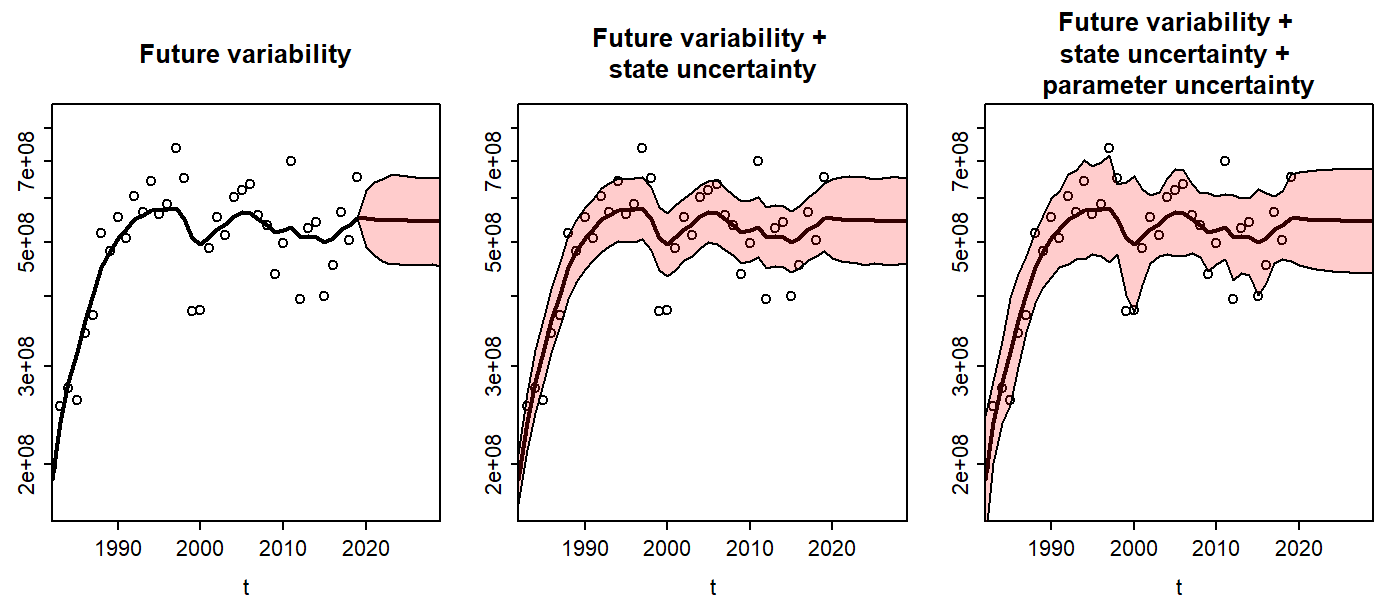
\includegraphics[width=5.5in]{Chap_3/gompertz_forecast.png}
    \label{fig:Chap3_gompertz_forecast}
\end{figure}

\section{Chapter Summary}

In summary, we have showed that:
\begin{enumerate}
    \item Population-dynamics models generally define a probability distribution for population growth rates based on the abundance in preceding times. A simple approximation to population dynamics results in the Gompertz population model, and this defines a first-order autoregressive process;

    \item If a stochastic population dynamics model is combined with a probability distribution for measurements of abundance, then the resulting ``state-space" model can be estimated by specifying process errors (or the state-variable) as a random effect;
    
    \item In an autoregressive model like Gompertz population dynamics, the degree of autoregression defines a ``semivariogram". If dynamics are stationary, this semivariance function can instead be represented as a covariance function. Similarly, an autoregressive model can be specified either by factoring the covariance of states into a series of conditional distributions or by constructing this joint covariance directly. Furthermore, it is more efficient to construct the joint precision directly than constructing the joint covariance and then have to invert it.  Joint and conditional covariance models can be specified to give identical results, or will sometimes differ slightly given small differences in implied boundary conditions;
    
    \item An autoregressive model generally has a sparse precision matrix for random effects, as can be shown by using automatic sparseness detection in TMB, using a graphical model to illustrate dependencies, or by deriving it from a simultaneous autoregressive process;
    
    \item It is straightforward to fit a state-space model given missing or unevenly spaced data. Similarly, forecasts involving a state-space model can decompose uncertainty into components representing future variability, uncertainty about historical states that define the initial conditions for a forecast, and parametric uncertainty, and all versions are straightforward to obtain using TMB. 
\end{enumerate}

\section{Exercise}

In Eq. \ref{eq:Chap3_IAR}, we introduce an IAR model by specifying the conditional distribution for each time \(t\) given the time \(t-1\) preceding it.  We also claimed that this IAR could instead be described by specifying the joint distribution for biomass at all modeled times, similar to what's done in Section \ref{sec:Chap3_joint_Gompertz}.  Please write down this joint specification of the IAR model, implement both in TMB, and confirm that both given similar results when applied to the flathead sole data set. 

